\chapter{O CERN e Física Experimental de Altas Energias}

Neste capítulo estão descritos com maiores detalhes o contexto no qual o
trabalho está inserido. Serão introduzidos o estudo de Física de Partículas
Elementares e o Modelo Padrão (seção \ref{sec:fis_part}),
 o experimento LHC (seção~\ref{sec:lhc}), o detetor ATLAS 
(seção~\ref{sec:ATLAS}), e o ferramental utilizado pela colaboração
(seção~\ref{sec:ferramentas}). 

\section{Física das Partículas Elementares}
\label{sec:fis_part}


\section{O Large Hadron Collider}
\label{sec:lhc}

%TODO Falar de luminosidade e coisas da introdução da tese do LAr

O CERN ({\it Centre Européene pour la Rechèrche Nucleaire}) é o maior
laboratório de física de partículas do mundo, situado na fronteira da Suíça com
a França, contando com a colaboração de cientistas vindos de institutos
do mundo todo. Desde sua fundação em 1954, tem sido uma das referências de
avanços tecnológicos. Dentre seus feitos constam a construção do primeiro 
colisionador de prótons-prótons (1971), a descoberta 
da corrente de neutrons (1973) e das partículas Z e W (1983), 
e a invenção da Web (1990) \cite{webCERN}.

Atualmente, o CERN está engajado no projeto LHC (Large Hadron
Collider), um acelerador de partículas circular de 27 quilômetros de
circunferência, que colide no atual momento feixes de prótons a uma energia
máxima de 7 TeV, sendo expandidos a 14 TeV em 2013 \cite{webATLAS}.
O LHC apresenta uma oportunidade sem precedentes para provar o domínio da
nova física na região TeV e lançar luz sobre algumas das questões fundamentais
não resolvidas da física das partículas elementares \cite{hunt_for_physics}. 

Para desenvolver a altíssima energia necessária para o experimento o CERN 
utiliza outros aceleradores construídos anteriormente, acelerando os feixes de prótons até atenderem
a energia desejada para a colisão. Na Figura \ref{fig:esquema_aceleradores} pode-se observar
o esquema de aceleração de prótons, inicia-se na extração de prótons de átomos
de hidrogeneo que são levados ao LINAC 2, um acelerador linear,
que inicia a sequencia de aceleração. Em seguida são utilizados os aceleradores
circulares BOOSTER, PS, SPS, até finalmente abastecer o LHC com os feixes de
prótons.

\begin{figure}[h!t]
\centering
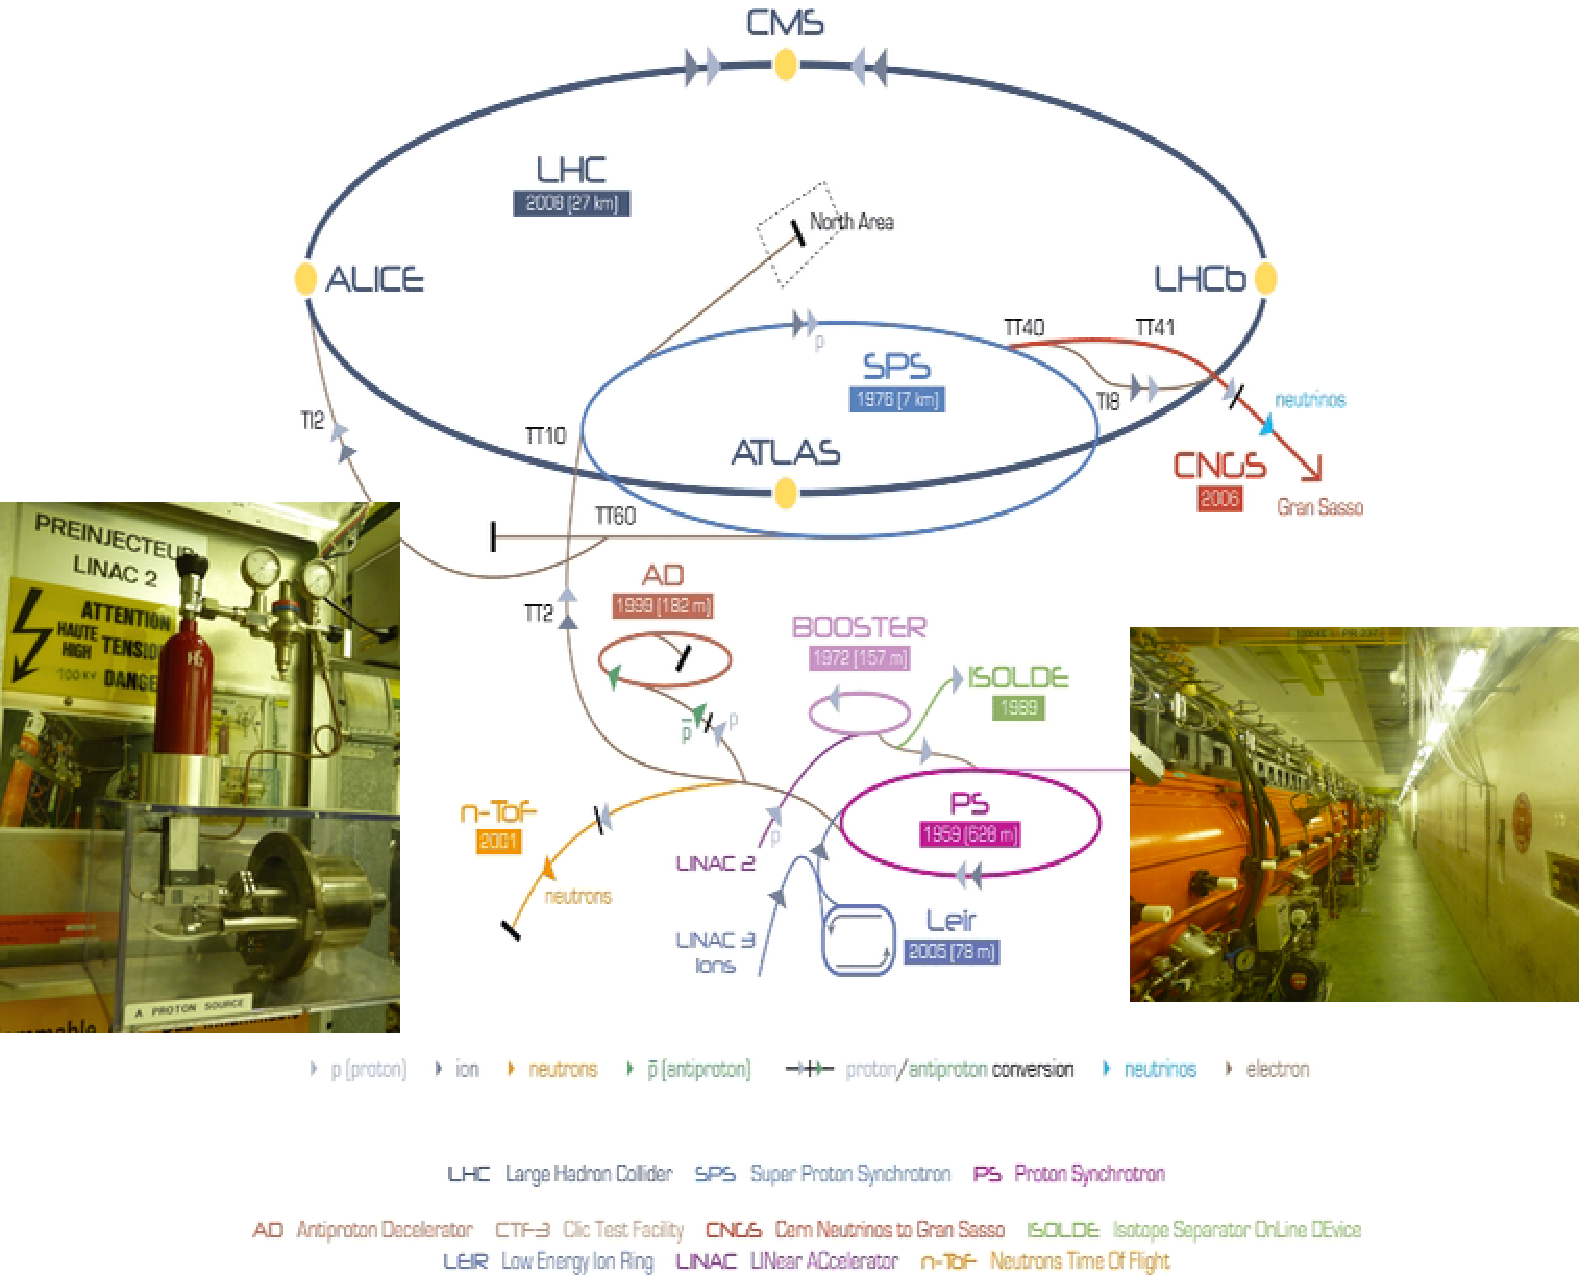
\includegraphics[width=\textwidth]{imagens/lhc_garrafa_linac2.pdf}
\caption{Os diferentes aceleradores e detectores do CERN, extraido de
\cite{cern_accelerators}. A seta cinza claro corresponde ao sentido do
deslocamento de prótons nos aceleradores. À esquerda, foto da garrafa
de onde são retirados os prótons, e na direita foto do LINAC 2.}
\label{fig:esquema_aceleradores}
\end{figure}

As colisões podem ser de dois tipos \cite{THESIS_LAR}:

\begin{enumerate}
\item \textbf{Colisões Rigidas}:
elas são devidas as interações de curto alcance,
resultando em grandes transferências de momemnto que produzindo partículas de
alto momento, assim como condições para a geração de novas partículas de altas energias.
\item \textbf{Colisões Suaves}: 
devidas as interações de longo alcance entre dois prótons cruzantes. Os
resultados são partículas com grande momentos longitudinais (na direção de
propagação do feixe) e pouco momento transverso. Esses eventos de colisão são
denominados de \emph{mininum bias} e são compostos na sua maioria por jatos.
\end{enumerate}

O experimento LHC conta com quatro detectores de maior escala: ATLAS, CMS, ALICE e
LHCb; e dois de menor escala: TOTEM e LHCf. O trabalho atual está definido no
escopo da colaboração do detector ATLAS, onde o mesmo é definido com maiores
detalhes na seção~\ref{sec:ATLAS}.

O ATLAS e o CMS são de propósito geral, ou seja, são capazes de estudar diversos
fenômenos físicos. O fato de existirem dois detectores projetados de forma
diferente, mas para o mesmo fim, é importante para que um possa confirmar o
resultado do outro.

O LHCb é um detector especializado no estudo do quark \textit{beauty} com o
intuito de investigar a diferença entre matéria e antimatéria.

O ALICE, por sua vez, estudará o plasma quark-gluon que será formado quando o
LHC fizer colisões de íons de chumbo, recriando as condições que existiram
instantes após o Big Bang.

Os dois menores detectores são o LHCf e o TOTEM. O LHCf, que se situa na mesma
caverna do ATLAS, estuda o comportamento de raios cósmicos, utilizando
partículas que não chegaram a colir no ponto de colisão, mas foram desviadas.
O TOTEM, que está instalado perto do CMS, estuda o feixe de prótons produzidos
pelo LHC, bem como a estrutura interna do próton.

\section{O Detector de Partículas ATLAS}
\label{sec:ATLAS}

O ATLAS (\textit{A Toroidal LHC Apparatus}) é o maior dos detectores que operam
no LHC, medindo 45 metros de comprimento e 25 metros de altura e largura. Como é
um detector de propósito genérico, o detector registra dados sobre os eventos de
colisões de partículas que podem ser usados para estudos em diversas áreas da
física. Um dos estudo mais esperados é o que comprova ou rejeita a existência do Bóson de
Higgs, confirmando a teoria que explica de onde vem a massa das partículas.

O experimento está na fase de operação desde setembro de 2008 \cite{webLHCFirstBeam},
quando o primeiro feixe de partículas circulou no acelerador e os primeiros
eventos de colisão dos prótons com moléculas de gás dentro do tubo do acelerador
foram registrados. Para coletar dados suficientes para as análises físicas o
experimento pode durar cerca de 20 anos \cite{ATLAS_TDR}.

O ATLAS foi construído e é operado por uma colaboração internacional envolvendo
cerca de 2500 físicos de mais de 169 instituições e laboratórios de 37 países
\cite{webATLAS}. Esses números incluem a UFRJ, que participa através da COPPE,
da Escola Politécnica e do Instituto de Física. O detector é composto por 4
sub-detectores: o Inner detector, detector de traço; o Liquid Argon, que é o
calorímetro eletromagnético; o Tile Calorimeter, que é o calorímetro hadrônico,
e o Muon Spectrometer responsável por realizar medições sobre os múons. Cada uma
dessas partes teve seus componentes construídos por um grupo diferente,
pertencente às instituições colaboradoras.  Uma vez construídos e testados, os
componentes foram levados ao CERN, onde foram instalados em seus lugares
definitivos. Para coordenar essa montagem e fornecer a infra-estrutura
necessária no local do experimento, existe o grupo da Coordenação Técnica
({\it ATLAS Technical Coordination}).

\section{Ferramentas Utilizadas na Colaboração}
\label{sec:ferramentas}

